\chapter{Algoritmo wavefront per la distanza di edit}
    La \textbf{complessità in tempo} (e \textbf{in memoria}) $\Theta(n m)$ rende poco pratico l'utilizzo dell'algoritmo di \textbf{Needleman-Wunsch} \cite{NeedlemanWunsch} su sequenze di grandi dimensioni; ciò risulta ancora più evidente nell'estensione dell'algoritmo sui \textbf{grafi di sequenza} (sezione \ref{section:poa-complexity}) e sui \textbf{grafi di variazione} (sezione \ref{section:variation-complexity}), limitando fortemente le dimensioni dei grafi che è possibile trattare in tempi realistici. Recentemente è stato ripreso e sviluppato \cite{WFA_edit-distance} un algoritmo per calcolare l'allineamento di sequenze in modo esatto, chiamato \textbf{\textit{wavefront algorithm} (WFA)} \cite{UKKONEN1985100}, che permette di computare la \textbf{distanza di edit} di \emph{due sequenze} con una complessità in tempo lineare rispetto alla dimensione delle sequenze e al valore ottimale della stessa \textbf{distanza di edit}: in questo capitolo si propone una trattazione formale dell'algoritmo e una sua possibile estensione sui \textbf{grafi di variazione}. 
\label{section:wfa}

\section{Algoritmo wavefront per la distanza di edit tra due sequenze}
    Quando si calcola la \textbf{distanza di edit} tra due sequenze utilizzando le equazioni descritte nella sezione \ref{section:edit-distance}, la \emph{matrice di programmazione dinamica} di dimensione $(n + 1) \times (m + 1)$ viene computata completamente, indipendentemente da quale sia il valore effettivo della \textbf{distanza di edit ottimale}:
\clearpage

    \begin{figure}[ht]
        \centering
        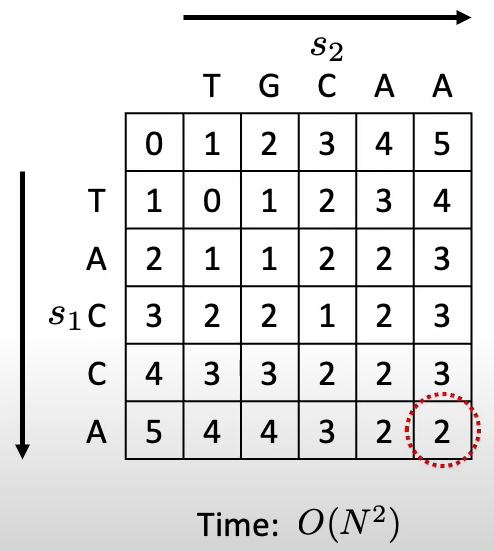
\includegraphics[width=0.5\textwidth]{images/wfa_complete_matrix.png}
        \caption{\emph{Matrice di programmazione dinamica} per il calcolo della \textbf{distanza di edit} tra due sequenze. \cite{wfa_sequence_graph}}
        \label{fig:wfa_complete_matrix}
    \end{figure}
    \vspace{20pt}
    Tuttavia, è possibile notare che tutte le celle che hanno un valore strettamente maggiore della \textbf{distanza di edit ottimale} non contribuiscono al calcolo della soluzione ottimale e, di conseguenza, non si troveranno mai nel percorso che porta alla soluzione migliore. Questa è una conseguenza diretta del fatto che l'algoritmo di programmazione dinamica della \textbf{distanza di edit} risolve un \emph{problema di minimizzazione} in cui le \emph{penalità} utilizzate sono \emph{strettamente positive}: di conseguenza, prese in ingresso le due sequenze $X_n = <x_1, x_2, ..., x_n>$ e $Y_m = <y_1, y_2, ..., y_m>$, vale la seguente proprietà:
    \begin{equation*}
        D[i, j] \geq D[i-1, j-1]
    \end{equation*}
    e, in particolare
    \begin{equation*}
       D[i, j] = D[i-1, j-1] \iff x_i = y_j
    \end{equation*}
    $$\forall i \in \{1, ..., n\}, \, \forall j \in \{1, ..., m\}$$
    Detto a parole, le \emph{diagonali} sono \emph{crescenti in senso lato} su tutta la matrice, e \emph{crescenti in senso stretto} se non sono presenti corrispondenze (\emph{match}) nelle sottostringhe considerate. L'idea dietro all'algoritmo \textbf{\textit{wavefront}} è di sfruttare questa proprietà per evitare di calcolare tutte le celle che corrispondono a una \textbf{distanza di edit} maggiore di quella ottimale: per far questo, gli indici e il contenuto della matrice di programmazione dinamica cambiano come segue:
    \begin{itemize}
        \item gli indici della matrice diventano la \emph{diagonale} che si sta computando e lo \textbf{distanza di edit} a cui si è arrivati;
        \item il valore degli elementi della matrice diventa il maggior \emph{offset} sulla \emph{diagonale} di interesse per la \emph{distanza di edit} considerata.
    \end{itemize}
    Si definisce \textbf{fronte d'onda} l'insieme composto dalle celle della matrice che hanno la stessa \emph{distanza di edit}: esse vengono computate tutte durante la medesima iterazione dell'algoritmo. E' possibile suddividere \textbf{\textit{WFA}} in due fasi principali:
    \begin{itemize}
        \item L'\textbf{estensione}, in cui tutte le diagonali appartenenti allo stesso \emph{fronte d'onda} vengono appunto "estese" il più possibile (fino a quando ci sono dei \textbf{match} tra i simboli delle sequenze); 
        \item L'\textbf{espansione}, in cui viene computato il \emph{fronte d'onda successivo} a partire dalle diagonali del \emph{fronte d'onda attuale}.
    \end{itemize}
    
    \begin{figure}[h]
        \centering
        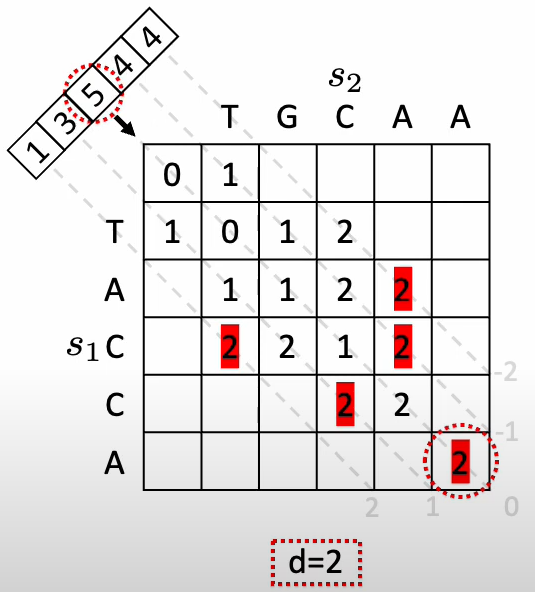
\includegraphics[width=0.5\textwidth]{images/wfa_partial_matrix.png}
        \caption{\emph{Matrice di programmazione dinamica} virtualmente computata da \textbf{\textit{WFA}}: i numeri in basso a destra rappresentano il numero della \emph{diagonale}, mentre quelli in alto a sinistra il valore degli \emph{offset} sulle rispettive \emph{diagonali}. \cite{wfa_sequence_graph}}
        \label{fig:wfa_partial_matrix}
    \end{figure}
    \vspace{20pt}

\subsection{Equazioni di ricorrenza}
    Da un punto di vista matematico, questo viene espresso dalle seguenti equazioni: siano

    \begin{itemize}
        \item $\Sigma$ l'\textbf{alfabeto} di definizione,
        \item  $X_n = <x_1, x_2, ..., x_n>, \, x_i \in \Sigma \, \, \forall i \in \{1, 2, ..., n\}$ la \textbf{prima sequenza},
        \item  $Y_m = <y_1, y_2, ..., y_m>, \, y_j \in \Sigma \, \, \forall j \in \{1, 2, ..., m\}$ la \textbf{seconda sequenza},
        \item $$D[i, j] = \begin{cases}
            D[i-1, j-1] & se \, \, x_i = y_j \\
            \min \begin{cases}
                D[i, j-1] & \\
                D[i-1, j-1] & \\
                D[i-1, j] & \\
            \end{cases} + 1 & se \, \, x_i \neq y_j 
        \end{cases}$$ la \emph{matrice di programmazione dinamica} computata dall'algoritmo standard per il calcolo della \textbf{distanza di edit} (sezione \ref{section:edit-distance});
    \end{itemize}

    Si definiscono
    \begin{itemize}
        \item $k = j - i$ come la \emph{k-esima diagonale},
        \item \begin{equation}
            H[d, k] = \begin{cases}
                max\{j \mid D[j - k, j] = d\}, & \, se \, \, \exists j \, s.t. \, D[j - k, j] = d \\
                -\infty, & altrimenti
            \end{cases}
        \label{equation:wf_extension_definition}
        \end{equation}
        come il valore del maggior \emph{offset} per la \emph{k-esima diagonale} tra le celle di programmazione dinamica con \textbf{distanza di edit} \emph{d} (dopo una fase di \textbf{estensione}).
        \item \begin{equation}
            J[d, k] = \begin{cases}
                min\{j \mid D[j - k, j] = d\}, & \, se \, \, \exists j \, s.t. \, D[j - k, j] = d \\
                -\infty, & altrimenti
            \end{cases}
        \label{equation:wf_expansion_definition}
        \end{equation}
        come il valore del minor \emph{offset} per la \emph{k-esima diagonale} tra le celle di programmazione dinamica con \textbf{distanza di edit} \emph{d} (dopo una fase di \textbf{espansione}).
    \end{itemize}
    Come conseguenza delle definizioni \ref{equation:wf_extension_definition} e \ref{equation:wf_expansion_definition} vale la seguente implicazione:
    \begin{equation*}
        D[j-k, j] = d \iff J[d,k] \leq j \leq H[d,k]
    \end{equation*}
    Ovvero l'\emph{offset} di qualsiasi cella con \textbf{distanza di edit} $d$ che si trova sulla diagonale $k$ è compreso tra  $J[d,k]$ e $H[d,k]$.
    
    Le due fasi di \textbf{estensione} ed \textbf{espansione} vengono descritte dalle seguenti equazioni di ricorrenza:
\subsubsection{Estensione del fronte d'onda}
    \begin{equation}
        H[d,k] = j + LCP(X[j - k + 1:], Y[j + 1:]), \quad j = J[d,k]
    \label{equation:wf-extension}
    \end{equation}
    dove
    $$LCP(x, y) = \lvert Longest \, Common \, Prefix(x, y) \rvert$$

\subsubsection{Espansione del fronte d'onda}
    \begin{equation}
        J[d, k] = max \begin{cases}
            H[d - 1, k - 1] + 1, \\
            H[d - 1, k] + 1, \\
            H[d - 1, k + 1]
        \end{cases}
    \label{equation:wf-expansion}
    \end{equation}

    Le equazioni \ref{equation:wf-extension} e \ref{equation:wf-expansion} esprimono l'alternarsi delle due fasi di \textbf{estensione} ed \textbf{espansione}: dopo aver computato tutti i \textbf{match} possibili, le diagonali vengono espanse per la \textbf{distanza di edit} successiva, per poi reiterare il procedimento.

\subsection{Condizioni al contorno}
    Le \textbf{condizioni al contorno} vengono riformulate come segue:

\subsubsection{Caso globale}
    \textbf{Caso base}:
    \begin{equation}
        H[0, 0] = 0
    \label{section:wfa_global_base_case}
    \end{equation}

    \textbf{Soluzione ottima}: $$d \, \, s.t \, \, H[d, m - n] = m$$
    
\subsubsection{Caso semiglobale}
    \textbf{Caso base}:
    \begin{equation}
        H[0, -i] = 0, \quad \forall i \in \{0, ..., n\} 
        \label{section:wfa_semiglobal_base_case}
    \end{equation}
    \textbf{Soluzione ottima}:
    $$d \, \, s.t \, \, H[d, m - i] = m, \quad \forall i \in \{0, ..., n\}$$

\subsection{Pseudocodice}
    Da un punto di vista algoritmico, le due procedure di \textbf{estensione} ed \textbf{espansione} vengono espresse tramite il seguente pseudocodice:
\subsubsection{Extend}
    \begin{algorithm}[H]
        \KwData{$X_n, Y_m, d, H_d$}
        \For{k = -d \KwTo d} {
            $i \gets H[d][k] - k$\;
            $j \gets H[d][k]$\;
            \While{$x_i = y_j$} {
                $i \gets i + $1\;
                $j \gets j + 1$\;
                $H[d][k] \gets H[d][k] + 1$\;
            }
        }
    \caption{extend}
    \label{alg:extend}
    \end{algorithm}
    Nell'estensione il numero di diagonali del \emph{d-esimo fronte d'onda} non cambia.
    
\subsubsection{Expand}
    \begin{algorithm}[H]
        \KwData{$X_n, Y_m, d, H_d$}
        \textbf{initialize} $H_{d+1}$\;
        $k_{lo} \gets -(d + 1)$\;
        $k_{hi} \gets d + 1$\;
        \For{k = $k_{lo}$ \KwTo $k_{hi}$} {
            $H[d + 1, k] \gets \max\{H[d, k - 1] + 1, \, H[d, k] + 1, \, H[d, k + 1]\}$\;
        }
        \caption{expand}
        \label{alg:wf_expand}
    \end{algorithm}
    Nella fase di espansione viene computato il \emph{fronte d'onda} successivo: è necessario considerare le due nuove diagonali $-(d+1)$ e $d+1$.
    
    \vspace{20pt}
    A seguire lo pseudocodice per la procedura  principale \textbf{\textit{WFA}} nella \textbf{modalità globale}:
\subsubsection{Caso globale}
    \begin{algorithm}[H]
        \caption{WFA\_global}
        \label{alg:wfa_global}
        \KwData{$X_n, Y_m$}
        \KwResult{$d = edit\_distance(X_n, Y_m)$}
        \textbf{initialize} $H_0$\;
        $H[0][0] \gets 0$\;
        $d \gets 0$\;
        \While{$true$}{
            $extend(X_n, Y_m, d, H_d)$\;
            \If{$H[d, m-n] = m$} {
                $break$\;
            }
            $expand(X_n, Y_m, d, H_d)$\;
            $d \gets d + 1$\;
          }
        $traceback(X_n, Y_m, d, H_d)$\;
        $return \, d$\;
    \end{algorithm}

    \vspace{20pt}
    E nella \textbf{modalità semiglobale}:
    
\subsubsection{Caso semiglobale}
    \begin{algorithm}[H]
        \caption{WFA\_semiglobal}
        \label{alg:wfa_semiglobal}
        \KwData{$X_n, Y_m$}
        \KwResult{$d = edit\_distance(X_n, Y_m)$}
        \textbf{initialize} $H_0$\;
        \For{i = 0 \KwTo n} {
            $H[0][-i] = 0$
        }
        $d \gets 0$\;
        \While{$true$}{
            $extend(X_n, Y_m, d, H_d)$\;
            \For{i = 0 \KwTo n} {
                \If{$H[d, m-i] = m$} {
                    $break$\;
                }
            }
            $expand(X_n, Y_m, d, H_d)$\;
            $d \gets d + 1$\;
          }
        $traceback(X_n, Y_m, d, H_d)$\;
        $return \, d$\;
    \end{algorithm}

    Si noti che nella \textbf{modalità semiglobale}, le sottoprocedure \textbf{extend} ed \textbf{expand} vanno modificate in maniera da considerare il range di diagonali $[-n, d]$ a ogni iterazione.
    \vspace{20pt}

    Infine un esempio (figura \ref{fig:wfa-example}) che mostra la \emph{matrice} computata da \textbf{\textit{WFA\_global}} e quella che verrebbe virtualmente calcolata dall'algoritmo standard:
    
    \begin{figure}[ht]
        \centering
        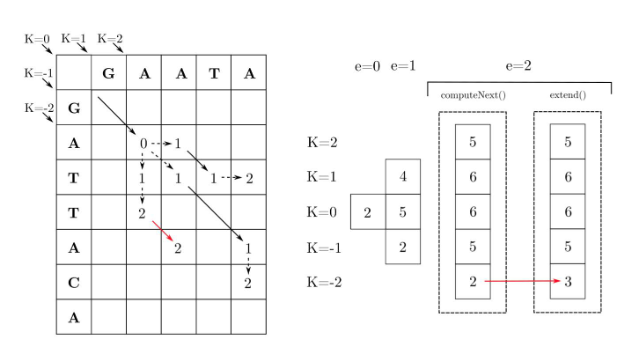
\includegraphics[width=1\textwidth]{images/wfa_example.png}
        \caption{Matrice effettivamente calcolata da \textbf{\textit{WFA}} rispetto a quella che verrebbe virtualmente computata dall'algoritmo standard. \cite{WFA_edit-distance}}
        \label{fig:wfa-example}
    \end{figure}

\subsection{Complessità computazionale}
    Si consideri la seguente notazione:
    \begin{itemize}
        \item $n$ = lunghezza della \emph{sequenza più lunga} \textbf{(testo)},
        \item $m$ = lunghezza della \emph{sequenza più corta} \textbf{(query)},
        \item $\overline{d}$ il valore ottimo della \textbf{distanza di edit} tra le due sequenze.
    \end{itemize}
    Si noti che la \textbf{distanza di edit} $d$ è \emph{limitata inferiormente} dalla differenza della lunghezza delle due sequenze ed è \emph{limitata superiormente} dalla lunghezza maggiore tra le sequenze:
    \begin{equation}
        n - m \leq \overline{d} \leq n
    \label{equation:edit-dist_limit}
    \end{equation}

\subsubsection{Complessità in tempo}
    La \textbf{complessità in tempo} di \textbf{\textit{WFA}} è determinata dalle operazioni presenti all'interno del ciclo principale, che viene eseguito una volta per ogni valore della \textbf{distanza di edit} $d \in \{0, 1, ..., \overline{d}\}$ e contenente le tre sottoprocedure:
    \begin{itemize}
        \item \textbf{extend},
        \item \textbf{controllo terminazione},
        \item \textbf{expand},
    \end{itemize}
    e dalla procedura \textbf{traceback}. Si procede a analizzare il tempo richiesto da ognuna delle sottoprocedure.
\subsubsection{Extend}
\begin{itemize}
    \item \textbf{Caso globale}: nella sottoprocedura \textbf{extend} (algoritmo \ref{alg:extend}) il tempo di esecuzione è proporzionale al numero totale di \textbf{match} effettuato da tutte le diagonali, appartenenenti all'insieme $\{-\overline{d}, -\overline{d} + 1, ..., 0, ..., \overline{d}-1, \overline{d}\}$.
        E' possibile distinguere due casi:
        \begin{itemize}
            \item $m \leq \overline{d} \leq n \implies m = O(\overline{d})$, rappresentato dalla seguente figura
            \vspace{20pt}
                \begin{figure}[h]
                    \centering
                    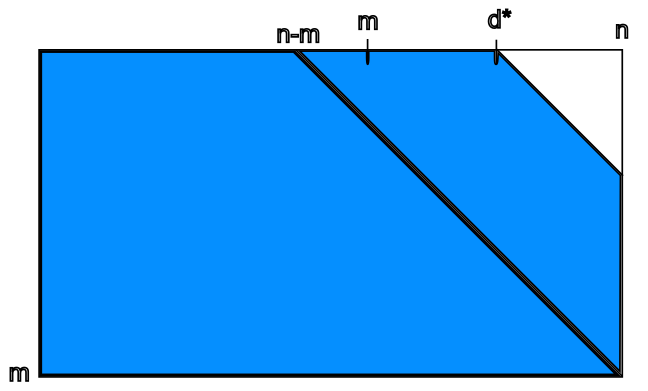
\includegraphics[width=0.7\textwidth]{images/wfa_extend_matrix_1.png}
                    \caption{Sezione della \emph{matrice di programmazione dinamica} in cui si possono verificare il massimo numero di \textbf{match} (caso $m \leq \overline{d} \leq n$).}
                    \label{fig:wf_extend_matrix_1}
                \end{figure}
    
                In questo caso il \emph{numero massimo} di \textbf{match} è dato da
                \begin{align*}
                    &T(n, m, \overline{d}) = \\ 
                    &= \sum_{j=0}^{m}{m-j}& &+& &\sum_{i=1}^{n-m}{m}& &+& &\sum_{i=1}^{\overline{d}-(n-m)}{m-i} = \\
                    &= \frac{m(m+1)}{2}& &+& &m(n-m)& &+& &\frac{(\overline{d}-(n-m)) (m+(n-\overline{d})-1)}{2}
                \end{align*}
                Per \ref{equation:edit-dist_limit} si ha che
                \begin{itemize}
                    \item $n-m \leq \overline{d} \implies n-m = O(\overline{d})$
                    \item  $n - \overline{d} \leq m \implies n-\overline{d} = O(m)$
                \end{itemize}
                e di conseguenza
                \begin{align*}
                    T(n, m, \overline{d}) = O(m^2) + O(m) \cdot O(\overline{d}) + O(\overline{d}) \cdot O(m) = O(m \cdot \overline{d})
                \end{align*}
                Si osservi che porre $n-m \leq m \leq \overline{d}$ non è limitante, in quanto è il caso in cui si considerano il maggior numero di diagonali (rispetto al caso $m \leq n-m \leq \overline{d}$ o al caso $m \leq \overline{d} \leq n-m$).
            
            \item $\overline{d} \leq m \leq n \implies m = O(\overline{d})$, rappresentato dalla seguente figura
            \vspace{20pt}
                \begin{figure}[h]
                    \centering
                    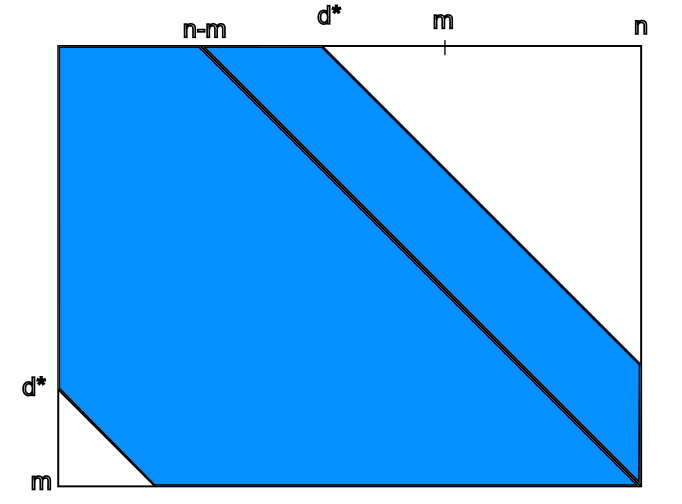
\includegraphics[width=0.7\textwidth]{images/wfa_extend_matrix_2.png}
                    \caption{Sezione della \emph{matrice di programmazione dinamica} in cui si possono verificare il massimo numero di \textbf{match} (caso $\overline{d} \leq m \leq n$).}
                    \label{fig:wf_extend_matrix_2}
                \end{figure}
                
                Per questa altra possibilità si nota che viene computata una sezione di \emph{matrice di programmazione dinamica} inferiore rispetto al caso precedente; quindi il tempo sarà sempre limitato da
                $$T(n, m, \overline{d}) = O(m \cdot \overline{d})$$
                Anche in questa casistica, porre $n-m \leq \overline{d} \leq m$ non è limitante.
        \end{itemize}
        Quindi, il tempo della sottoprocedura \textbf{extend} nel \textbf{caso globale} è \emph{limitato superiormente} da
        $$T(n, m, \overline{d}) = O(\min\{n, m\} \cdot \overline{d})$$
        
    \item \textbf{Caso semiglobale}: in questa modalità, vengono considerate tutte le diagonali $k \in \{0, -1, ..., -n\}$      fin dalla prima iterazione; di conseguenza, il tempo di esecuzione risulta:
        \begin{align*}
                    &T(n, m, \overline{d}) = \\ 
                    &= \sum_{j=0}^{\overline{d}}{m-j}& &+& &\sum_{i=1}^{n-m}{m}& &+& &\sum_{i=1}^{n-(n-m)}{m-i} = \\
                    &= \frac{(\overline{d}+1) \cdot (2m -\overline{d})}{2}& &+& &m(n-m)& &+& &\frac{m(m-1)}{2}
                \end{align*}
        ovvero
        \begin{equation*}
            T(n, m, \overline{d}) = O(m \cdot (\overline{d} + m))
        \end{equation*}
         
    \end{itemize}

\subsubsection{Controllo terminazione}
    \begin{itemize}
        \item Per quanto riguarda il \textbf{caso globale} (algoritmo \ref{alg:wfa_global}), il \textbf{controllo di terminazione} viene effettuato in tempo costante: 
        $$T(n, m, \overline{d}) = O(1)$$
        \item Nel \textbf{caso semiglobale} (algoritmo \ref{alg:wfa_semiglobal}), invece, è necessario controllare a ogni iterazione gli offset di tutte le diagonali corrispondenti a una posizione della sequenza più lunga (chiamata \textbf{testo}); il tempo risulta quindi essere 
        $$T(n, m, \overline{d}) = O(\max\{n, m\} \cdot \overline{d})$$ 
    \end{itemize}

\subsubsection{Expand}
    \begin{itemize}
        \item \textbf{Caso globale}: nella sottoprocedura \textbf{expand} (algoritmo \ref{alg:wf_expand}) ad ogni iterazione vengono effettuate $O(2d+1)$ operazioni: di conseguenza, la complessità temporale risulta essere limitata da $O(\sum_{d=0}^{\overline{d}}{2d+1}) = O(\overline{d} \cdot (\overline{d}+2)) = O(\overline{d}^2)$, ovvero:
        $$T(n, m, \overline{d}) = O(\overline{d}^2)$$

        \item \textbf{Caso semiglobale}: come succede nella \textbf{extend}, anche qui è necessario considerare tutte le diagonali $k \in \{0, -1, ..., -n\}$ fin dalla prima iterazione; il tempo risulta quindi $O(\sum_{d=0}^{\overline{d}}{d+n}) = O(\max\{n, m\} \cdot \overline{d}) + O(\overline{d}^2)$, ossia
        \begin{equation*}
            T(n, m, \overline{d}) = O(\max\{n, m\} \cdot \overline{d})
        \end{equation*}
    \end{itemize}
   

\subsubsection{Traceback}
    Come nel calcolo della \textbf{distanza di edit} standard, il tempo richiesto per ricostruire la soluzione è
    $$T(n, m, \overline{d}) = O(n + m)$$
    per entrambe le modalità.
    
    \vspace{20pt}
    La \textbf{complessità in tempo} totale risulta quindi essere:
    \begin{itemize}
        \item \textbf{Caso globale}:
        \begin{align*}
            T(n, m, \overline{d}) &= O(\min\{n, m\} \cdot \overline{d} + O(1) + O(\overline{d}^2) + O(n + m)) = \\
                                  &= O(\min\{n, m\} \cdot \overline{d} + \overline{d}^2 + (n + m))
        \end{align*}
        se interessati anche alla \textbf{ricostruzione della soluzione}, altrimenti
        \begin{equation}
            T(n, m, \overline{d}) = O(\min\{n, m\} \cdot \overline{d} + \overline{d}^2)
            \label{equation:wfa_global_time_complexity}
        \end{equation}
        \item \textbf{Caso semiglobale}:
        \begin{equation*}
            T(n, m, \overline{d}) = O(m \cdot (m + \overline{d})) + 2 \cdot O( \max\{n, m\} \cdot \overline{d}) + O(n + m)
        \end{equation*}
        ossia
        \begin{equation}
            T(n, m, \overline{d}) = O(\max\{n, m\} \cdot \overline{d})
             \label{equation:wfa_semiglobal_time_complexity}
        \end{equation}
    \end{itemize}

\subsubsection{Complessità in spazio}
    \begin{itemize}
        \item \textbf{Caso globale}: per quanto riguarda la \textbf{complessità in spazio}, ogni \emph{fronte d'onda} ha una dimensione proporzionale a $2d + 1$, con $d$ che varia da 0 a $\overline{d}$; di conseguenza, la \textbf{complessità spaziale}\footnote{Se non interessati alla \textbf{ricostruzione della soluzione}, la complessità scende a $M(n, m, \overline{d}) = O(\overline{d})$.} nel \textbf{caso globale} è data da
        \begin{equation}
            M(n , m, \overline{d}) = O(\overline{d}^2)
        \label{equation:wfa_global_space_complexity}
        \end{equation}

        \item \textbf{Caso semiglobale}: in questa modalità, vale la stessa osservazione del \textbf{caso globale}; tuttavia, è necessario considerare anche le diagonali $k \in \{0, -1, ..., -n\}$ fin dalla prima iterazione. La \textbf{complessità in spazio}\footnote{Se non interessati alla \textbf{ricostruzione della soluzione}, la complessità scende a $M(n, m, \overline{d}) = O(\max\{n, m\})$.} diventa quindi limitata da $O(\sum_{d=0}^{\overline{d}}{d+n}) = O(\max\{n, m\} \cdot \overline{d}) + O(\overline{d}^2)$, e di conseguenza
        \begin{equation}
            M(n , m, \overline{d}) = O(\max\{n, m\} \cdot \overline{d})
        \label{equation:wfa_semiglobal_space_complexity}
        \end{equation}
        
    \end{itemize}
    

\subsection{Dimostrazione di correttezza}
    Si considerino due \textbf{sequenze} $X_n = <x_1, x_2, ..., x_n>$ e $Y_m = <y_1, y_2, ..., y_m>$; la \textbf{distanza di edit} tra qualsiasi coppia di \textbf{prefissi} $X[:i]$, $Y[:j]$ è descritta dalla seguente equazione
    
    \begin{equation*}
        D[i,j] = \min \begin{cases}
            D[i-1,j] + 1 \\
            D[i-1,j-1] + \Delta_{i,j} \\
            D[i,j-1] + 1 \\
        \end{cases}
    \end{equation*}
    
    $$\Delta_{i,j} = \begin{cases}
        0 & \text{se }x_i = y_j \\
        1 & altrimenti
    \end{cases}$$
    che è \textbf{equivalente} alle seguenti equazioni
    
    \begin{equation}
        J[d,k] = \max \begin{cases}
            H[d-1, k + 1] \\
            H[d-1, k] + 1 \\
            H[d-1, k - 1] + 1 \\
        \end{cases}    
        \label{equation:expansion_demonstration}
    \end{equation}
        
    \begin{equation}
        H[d, k] = j + LCP(X[j - k + 1:], Y[j + 1:]), \quad j = J[d, k]
        \label{equation:extension_demonstration}
    \end{equation}
    con
    $$LCP(X, Y) = \lvert Longest \, Common \, Prefix (X, Y) \rvert$$

    Dove $H[d, k]$ è il \textbf{maggior offset} sulla \textbf{diagonale} $k = j - i$ per lo \textbf{score} $d$, definito come segue:
    \begin{equation}
        H[d, k] = \begin{cases}
            max\{j \mid D[j - k, j] = d\}, & \, se \, \, \exists j \text{ s.t. } D[j - k, j] = d \\
            - \infty, & \, altrimenti
        \end{cases}
    \label{equation_wf_h_correcteness}
    \end{equation}
    E $J[d, k]$ è il \textbf{minor offset} sulla \textbf{diagonale} $k = j - i$ per lo \textbf{score} $d$:
    \begin{equation}
        J[d, k] = \begin{cases}
            min\{j \mid D[j - k, j] = d\}, & \, se \, \, \exists j \text{ s.t. } D[j - k, j] = d \\
            - \infty, & \, altrimenti
        \end{cases}
    \label{equation_wf_j_correcteness}
    \end{equation}
    \textbf{Dimostrazione:} \\
    come conseguenza delle definizioni \ref{equation_wf_h_correcteness} e \ref{equation_wf_j_correcteness}, vale la seguente implicazione:
    \begin{equation}
        D[j - k, j] = d \iff J[d, k] \leq j \leq H[d, k]
        \label{equation:demonstration_property}
    \end{equation}
    Si definisca 
    \begin{equation}
        F[d, k, l] = \begin{cases}
            \max \{j \mid D[i, j] = d, j \leq l \}, & se \, \, \exists j \, s.t. \, D[i,j] = d \\
            - \infty, & altrimenti
        \end{cases}
    \end{equation}
    come il \textbf{maggior offset} sulla \textbf{diagonale} $k$ per lo \textbf{score} $d$ \emph{vincolato a essere minore o uguale} di $l$; come conseguenza della definizione, valgono le seguenti proposizioni:
    
    \begin{itemize}
        \item \textbf{Proposizione 1}
        \begin{equation}
            D[j-k, j] = d \iff F[d, k, j] = j
            \label{equation:demonstration_property_1}
        \end{equation}
         
        analoga a \ref{equation:demonstration_property} per $F[d,k,l]$
        
        \item \textbf{Proposizione 2}
        $$F[d, k, l] \leq F[d, k, l + 1]$$
        
        \item \textbf{Proposizione 3}
        $$J[d, k] = \min_l \{ F[d, k, l] \}$$
        $$H[d, k] = \max_l \{ F[d, k, l] \}$$
    \end{itemize}
    E' quindi possibile riscrivere le equazioni \ref{equation:expansion_demonstration} e \ref{equation:extension_demonstration} come
    
    \begin{equation}
        F[d,k,j] = \begin{cases}
             F[d,k,j-1] + 1, & \, if \, x_{j - k} = y_{j} \\
             max \begin{cases}
                F[d-1, k-1, j-1] + 1 \\
                F[d-1, k, j-1] + 1 \\
                F[d-1, k+1, j]
            \end{cases} & \, if \, x_{j - k} \neq y_{j}
        \end{cases}
    \end{equation}
    Infatti, in caso di \textbf{mismatch} ($x_i \neq y_j$), $F[d,k,j]$ viene computato a partire dagli offset per lo score $d-1$, come succede in \ref{equation:expansion_demonstration}; invece, in caso di \textbf{match} ($x_i = y_j$), $F[d,k,j]$ viene calcolato unicamente dagli offset per lo stesso score $d$; questo continua ad accadere finchè $x[j - k + q] = y[j + q]$, con $q \in \{0, ..., LCP(X[j - k + 1:], Y[j + 1:])$, in maniera analoga a \ref{equation:extension_demonstration}.
    
    Per \textbf{ipotesi di induzione} siano noti
    \begin{itemize}
        \item $F[d, k, j] = j$, il maggior offset sulla diagonale $k$ per lo score $d$ vincolato a essere minore o uguale a $j$
        
        \item $D[i, j] = d$, il valore ottimo della distanza di edit tra $X[:i]$ e $Y[:j]$
    \end{itemize}
    Sono possibili in tutto 4 casi:
    \begin{itemize}
        \item \textbf{Match: } $x_{i+1} = y_{j+1}$ \\
        In questo caso, il valore della distanza di edit resta invariato 
        $$D[i+1, j+1] = D[i,j] = d$$
        e l'offset sulla diagonale $k$ per lo score $d$ aumenta di uno
        $$F[d, k, j + 1] = F[d, k, j] + 1 = j + 1$$
        per \ref{equation:demonstration_property_1} vale
        $$F[d,k,j+1] = j + 1 \implies D[(j+1) - k, j+1] = d$$
        ossia
        $$D[(j+1)-k, j+1] = D[(j-k)+1, j+1] = D[i+1, j+1] = d$$
        
        \item \textbf{Mismatch: } $x_{i+1} \neq y_{j+1}$ \\ 
        In questo caso ci sono 3 possibilità:
    
        \begin{itemize}
            \item \textbf{Sostituzione}, ovvero si sostituisce $x_{i+1}$ con $y_{j+1}$, di conseguenza
            $$D[i+1, j+1] = D[i,j] + 1 = d + 1$$
            e l'offset sulla diagonale $k$ per lo score $d+1$ aumenta di uno
            $$F[d+1,k,j+1] = F[d,k,j] + 1 = j + 1$$
            per \ref{equation:demonstration_property_1} vale
            $$F[d+1,k,j+1] = j + 1 \implies D[(j+1)-k, j+1] = d + 1$$
            ossia
            $$D[(j+1)-k, j+1] = D[(j-k)+1, j+1] = D[i+1, j+1] = d + 1$$
    
            \item \textbf{Inserimento}, ovvero si inserisce $y_{j+1}$ dopo $X[:i]$, di conseguenza
            $$D[i,j+1] = D[i,j+1] + 1 = d + 1$$
             e l'offset sulla diagonale $k + 1$ per lo score $d+1$ aumenta di uno
            $$F[d+1,k+1,j+1] = F[d,k,j] + 1 = j + 1$$
            per \ref{equation:demonstration_property_1} vale
            $$F[d+1,k+1,j+1] = j + 1 \implies D[(j+1)-(k+1), j+1] = d + 1$$
            ossia
            $$D[(j+1)-(k+1), j+1] = D[(j-k)+1-1, j+1] = D[i, j+1] = d + 1$$
    
            \item \textbf{Cancellazione}, ovvero $x_{i+1}$ viene cancellato, di conseguenza
            $$D[i+1, j] = D[i,j] + 1 = d + 1$$
            e l'offset sulla diagonale $k - 1$ per lo score $d+1$ resta invariato
            $$F[d+1,k-1,j] = F[d,k,j] = j$$
            per \ref{equation:demonstration_property_1} vale
            $$F[d+1,k-1,j] = j \implies D[j-(k-1), j] = d + 1$$
            ossia
            $$D[j-(k-1), j] = D[(j-k)+1, j] = D[i+1, j] = d + 1$$
        \end{itemize}
    \end{itemize}

    Non esistono altre possibilità, quindi i quattro casi elencati coprono tutte le
    casistiche.

\subsection{Caso pesato}
    Risulta abbastanza immediato generalizzare l'algoritmo per l'utilizzo di \emph{penalità generiche}. \cite{Eizenga_wfa}
    
    Considerate in ingresso
    \begin{itemize}
        \item \textbf{\textit{ins}} = penalità per un \emph{inserimento},
        \item \textbf{\textit{m}} = penalità per una \emph{sostituzione},
        \item \textbf{\textit{del}} = penalità per una \emph{cancellazione},
    \end{itemize}
    con $(ins, m, del) \in \mathbb{Q}^3_+$, è possibile riscrivere l'equazione \ref{equation:wf-expansion} come:
    \begin{equation}
        J[d, k] = max \begin{cases}
            H[d - ins, k - 1] + 1 \\
            H[d - m, k] + 1 \\
            H[d - del, k + 1]
        \end{cases}
    \label{equation:wf-expansion_weighted}
    \end{equation}

    Per quanto riguarda lo pseudocodice, l'unica procedura a essere modificata è \textbf{expand} (algoritmo \ref{alg:wf_expand}):
    \begin{algorithm}[H]
        \KwData{$X_n, Y_m, d, H_d, ins, m, del$}
        \textbf{initialize} $H_{d+1}$\;
        $k_{lo} \gets -(d + 1)$\;
        $k_{hi} \gets d + 1$\;
        \For{k = $k_{lo}$ \KwTo $k_{hi}$} {
            $H[d + 1, k] \gets \max\{H[d + 1 - ins, k - 1] + 1, \, H[d + 1 - m, k] + 1, \, H[d + 1 - del, k + 1]\}$\;
        }
        \caption{expand}
        \label{alg:wf_expand_weighted}
    \end{algorithm}
    
\section{Estensione della distanza di edit tra grafo di variazione e sequenza con wavefront}

    Sfuttando la proprietà dei \textbf{grafi di variazione} di presentare \emph{percorsi lineari} (sezione \ref{section:variation_graph}), è possibile estendere l'approccio \textbf{\textit{wavefront}} su queste strutture dati\footnote{Diverse estensioni su \textbf{grafi di sequenza} (come \cite{wfa_POA_extension}) e \cite{wfa_sequence_graph}) sono già state proposte e sviluppate da diversi autori.}, aggiungendo alle \emph{matrici di programmazione dinamica} una dimensione per memorizzare i diversi percorsi.

\subsection{Equazioni di ricorrenza}
    Si considerino in ingresso
    \begin{itemize}
        \item un \textbf{grafo di variazione canonico} $G = (V, E, \delta, P)$, dove
        \begin{itemize}
             \item $V = \{v_0, v_1, v_2, ..., v_n\}$ è l'insieme dei \textbf{vertici} del grafo;
            \item  $E \subseteq V \times V$ è l'insieme degli \textbf{archi} del grafo;
            \item $\delta: V \rightarrow \Sigma$ è la \textbf{funzione di etichettatura}, 
            \item $P = \{p_1, p_2, ..., p_k\}, \, p_i = <v_0 = v_{i_1}, v_{i_2}, ..., v_{i_l} = v_n> \, \forall i \in \{1, 2, ..., k\}$ è l' \textbf{insieme dei percorsi del grafo}.  
        \end{itemize}
        \item una \textbf{sequenza} $Y_m = <y_1, y_2, ..., y_m>$;
        \item le \emph{penalità} di \textbf{inserimento}, \textbf{sostituzione} e \textbf{cancellazione }$(ins, m, del)$.
    \end{itemize}
    e si defnisca il \emph{suffisso di un cammino} come
    \begin{equation*}
        p[j:] = \delta(p_j) \delta(p_{j+1}) ... \delta(p_n)
    \end{equation*}
    $$\forall p \in P, \, \, \forall j \in \{0, ..., \lvert p \rvert\}$$
    Le equazioni \ref{equation:wf-extension} e \ref{equation:wf-expansion} possono essere riformulate come segue:
\subsubsection{Estensione del fronte d'onda}
    \begin{equation}
        H[d,k,p] = j + LCP(p[j - k + 1:], Y[j + 1:]), \quad i = J[d,k]
    \label{equation:wf_variation_extension}
    \end{equation}
    dove
    $$LCP(x, y) = \lvert Longest \, \, Common \, \, Prefix(x, y) \rvert$$

\subsubsection{Espansione del fronte d'onda}
    \begin{equation}
        J[d, k, p] = max \begin{cases}
            H[d - ins, k - 1, p] + 1, \\
            H[d - m, k, p] + 1, \\
            H[d - del, k + 1, p]
        \end{cases}
    \label{equation:wf_variation_expansion}
    \end{equation}

\subsection{Condizioni al contorno}
    Allo stesso modo, anche le condizioni al contorno \ref{section:wfa_global_base_case} e \ref{section:wfa_semiglobal_base_case} possono essere riscritte come:

\subsubsection{Caso globale}
    \textbf{Caso base}:
    \begin{equation}
        H[0, 0, p] = 0, \quad \forall p \in P 
        \label{section:wfa_variation_global_base_case}
    \end{equation}
    \textbf{Soluzione ottima}:
    \begin{equation}
        \min_{p \in P} \begin{cases}
            d \, \, s.t. \, \, H_{d, m-n, p} = m
        \end{cases}
        \label{section:wfa_variation_global_optimal}
    \end{equation}

\subsubsection{Caso semiglobale}
    \textbf{Caso base}:
    \begin{equation}
        H[0, -i, p] = 0, \quad \forall i \in \{0, ..., n\}, \, \forall p \in P 
        \label{section:wfa_variation_semiglobal_base_case}
    \end{equation}
    \textbf{Soluzione ottima}:
    \begin{equation}
        \min_{p \in P} \begin{cases}
            d \, \, s.t. \, \, H_{d, m-i, p} = m &  \forall i \in \{0, ..., n\}
        \end{cases}
        \label{section:wfa_variation_semiglobal_optimal}
    \end{equation}

\subsection{Complessità computazionale}
    Ogni percorso viene computato in maniera indipedente dagli altri, mantenendo la stessa complessità dell'allineamento tra due stringhe;
    
    Considerando la notazione 
    \begin{itemize}
        \item $n = \frac{\sum_{p \in P}{\lvert p \rvert}}{\lvert P \rvert}$, \emph{lunghezza media} dei \emph{percorsi} del \textbf{grafo di variazione},
        \item $m$ = lunghezza della \emph{sequenza} \textbf{(query)},
        \item $\overline{d}$ = valore ottimo della \textbf{distanza di edit} tra uno dei cammini del grafo e la sequenza,
        \item $p$ = numero dei \emph{percorsi} del \textbf{grafo di variazione},
    \end{itemize}
    la complessità per questo tipo di allineamento risulta:

\subsubsection{Caso globale}
    \textbf{Tempo:}
    \begin{equation}
            T(n, m, \overline{d}) = O((\min\{n, m\} + \overline{d}) \cdot \overline{d} \cdot p)
        \label{equation:wfa_variation_global_time_complexity}
        \end{equation}
    \textbf{Spazio:}
    \begin{equation}
        M(n , m, \overline{d}) = O(\overline{d}^2 \cdot p)
    \label{equation:wfa_variation_global_space_complexity}
    \end{equation}
        
\subsubsection{Caso semiglobale}
    \textbf{Tempo:}
    \begin{equation}
        T(n, m, \overline{d}) = O(n \cdot \overline{d} \cdot p)
    \label{equation:wfa_variation_semiglobal_time_complexity}
    \end{equation}

    \textbf{Spazio:}
    \begin{equation}
        M(n , m, \overline{d}) = O(n \cdot \overline{d} \cdot p)
    \label{equation:wfa_variation_semiglobal_space_complexity}
    \end{equation}

    Si noti che gli allineamenti tra i diversi cammini sono del tutto \emph{indipendenti} e quindi possono essere facilmente \emph{parallelizzati}.